\documentclass{article}

\usepackage{graphicx}
\usepackage{hyperref}
\usepackage{bm}
\usepackage{float}
\restylefloat{table}

\usepackage{listings}
\usepackage{color}
\usepackage{amsmath}

\usepackage[margin=1.25in]{geometry}

\definecolor{dkgreen}{rgb}{0,0.6,0}
\definecolor{gray}{rgb}{0.5,0.5,0.5}
\definecolor{mauve}{rgb}{0.86,0.27,0.22}

\lstset{frame=tb,
  language=python,
  aboveskip=3mm,
  belowskip=3mm,
  showstringspaces=false,
  columns=flexible,
  basicstyle={\small\ttfamily},
  numbers=left,
  stepnumber=1,
  numberstyle=\tiny\color{gray},
  keywordstyle=\color{blue},
  commentstyle=\color{dkgreen},
  stringstyle=\color{mauve},
  breaklines=true,
  breakatwhitespace=true,
  tabsize=3
}

\title{CS5200: Final Exam} % Title of the assignment

\author{Matthew Whitesides\\ \texttt{mbwxd4@umsystem.edu}} % Author name and email address

\date{\today} % University, school and/or department name(s) and a date

%----------------------------------------------------------------------------------------

\begin{document}

  \maketitle % Print the title

  \textit{I, Matthew Whitesides, certify that all the material in this PDF file is my original work, that I did not discuss these questions with anyone other than my instructor, and that I did not copy work from anyone for this examination.}
 
  \begin{enumerate}
    \item \textbf{Hamiltonian Paths and Cycles}.
    
    Please refer to the following labled nodes version of the graph for some of the questions.\\
    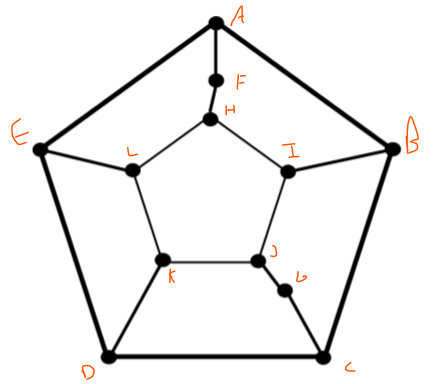
\includegraphics[scale=0.75]{1_Graph.png}

    \begin{enumerate}
        \item A Hamiltonian Path is defined as, "a graph path between two vertices of a graph that visits each vertex exactly once". Which yes this graph does have at least one. 
        
        For example the path in the labeled version above: 
        
        ${A \rightarrow F \rightarrow H \rightarrow I \rightarrow B \rightarrow C \rightarrow G \rightarrow J \rightarrow K \rightarrow D \rightarrow L}$ 
        
        would be a Hamiltonian Path.

        \item A Hamiltonian Cycle is defined as, " is a graph cycle (i.e., closed loop) through a graph that visits each node exactly once.".
        
        Given a node has to be used once, each node that has a degree of 2 would have to have both of it's edges used therefore edges (A,F),(F, H) and (J, G)(G, C) must be part of our cycle if one exists. 
        
        However if we must include these four edges note that no matter which direction we attemt to get to verticies (A, H) and (J, G) we form a closed subcircuit. 
        See the graph below to demonstrate this note the blue are edges we know must be in there and red and orage are two possible paths to those edges and both form a closed loop without including all the other verticies.

        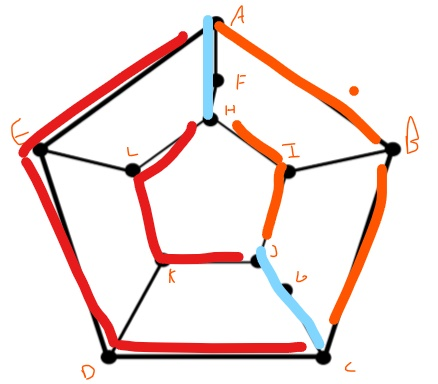
\includegraphics[scale=0.3]{1_Graph2.jpg}

        Therefore we know that this graph has no Hamiltonian cycle.

        \item
        \begin{itemize}          
          \item \textbf{The Problem.}
          \begin{itemize}
            \item We want to prove an n-dimensional cube contains a Hamiltonian Cycle. 
            \item An n-dimensional cube is defned as follows. It consists of the 2n vertices of the form $(a_0, a_1, ..., a_n)$ where each $a_i$ is either 0 or 1.
            \item Hamiltonian Cycle is defined as, " is a graph cycle (i.e., closed loop) through a graph that visits each node exactly once.".
            \item Our domain of n is any positive natual number in $n \ge 2$. As 0 would mean no edges or verticies and would be nothing, 1 would just be a line of two verticies which would not contain any cycles therefore not Hamiltonian, and a negitive numbers of edges does not make sense.
          \end{itemize}
          \item \textbf{Check the base case plus two others}.
          \begin{itemize}
            \item Base case: $n = 2$: This is true as this is just a square with 4 verticies and 4 edges, and if you simply use every edge you have formed a Hamiltonian cycle.
            \item $n = 3$: This would form a cube which we could represnt with the following graph: 
            
            
          \end{itemize}
        \end{itemize}

        
    \end{enumerate}

    \item \textbf{General Graph Theory}.
    \begin{enumerate}
        \item ToDo.
        \item Let's try a bit of a backword induction approach.
        
        If there are $N = 2$ people at the party then each person would have shaken hands with $(N - 1)$ person, e.g. the person other than John shook hands with one person which must be John.

        So if $Q(n)$ is out problem given $n$ people how many hands did John shake then $Q(2) = 1$.

        Now if $N = 3$ than we have John and two others which at most could have shaken hands with $(N - 1)$ person so the other handshakes would be $(N - 1), (N - 2)$ or $(2),(1)$.
        
    \end{enumerate}

    \item \textbf{NP Complete Problems}.
    \item \textbf{Red-Black Trees, B-Trees, and Binary Search Trees}.
    \item \textbf{More Graph Algorithms}.
    \item \textbf{GCD}.
  \end{enumerate}  % End of questions.
\end{document}
